% THIS GUIDE IS DESIGNED TO FULFILL THE FORMATTING REQUIREMENTS OF WICHITA STATE UNIVERSITY.
%============================================================================================================
% DEFINES THE DOCUMENT AS HAVING 12 POINT FONT, USES LETTERPAPER (8.5 X 11 INCHES), AND ENGLISH.
\documentclass[12pt,letterpaper,english]{article}

% PREAMBLE OF THE DOCUMENT, INCLUDES NUMEROUS PACKAGES TO MAKE THINGS GO SMOOTHLY AND ADD MORE FUNCTIONALITY

% MATH PACKAGE FOR EQUATIONS
\usepackage{amsmath}

% BETTER HANDLING OF GRAPHICS. USE .JPG, .EPS, OR .PNG FOR YOUR FIGURES. 
\usepackage{graphicx}

% ALLOWS SINGLE, DOUBLE, AND ONE HALF SPACING
\usepackage{setspace}

% SECTSTY ALLOWS THE ALTERATION OF SECTION STYLES AND TABLE OF CONTENTS PROPERTIES
\usepackage{sectsty}

% PROVIDES INDENTATION WHEN ENTERING TEXT AFTER A SECTION
\usepackage{indentfirst}

% TOCLOFT GIVES GREATER CONTROL OVER THE TABLE OF CONTENTS, FIGURES, AND TABLES
%\usepackage{tocloft}

% ENABLES SUBFIGURE USAGE
%\usepackage[tight]{subfigure}
\usepackage[subfigure]{tocloft}

% MULTIROW AND BOOKTABS PROVIDE EXTRA FUNCTIONALITY FOR TABLES
% CAPTION LETS YOU PUT CAPTIONS ON TOP OF TABLES

\usepackage{multirow}
\usepackage{booktabs}
\usepackage{caption}

%More additions
\usepackage{amssymb}
\usepackage{subfig}
\usepackage{algorithmic, algorithm2e}
\usepackage{listings}
\usepackage[sorting=none]{biblatex}
\usepackage{float}
\restylefloat{figure}
\nofiles

%TIMES NEW ROMAN FONT
\usepackage{times}

%\usepackage[american]{babel}
%\usepackage{csquotes}
%
%============================================================================================================
% END OF PACKAGE DECLARATIONS, NOW ONTO ALTERING THE DOCUMENT

% SETS THE DISTANCE BETWEEN FLOATS (TABLES AND FIGURES) AND TEXT
\setlength{\textfloatsep}{1.5ex}

% CAPTION TEXT SPACING AND LOCATION USING THE CAPTION PACKAGE
\DeclareCaptionLabelSeparator{lines}{\par\medskip}
\captionsetup[table]{labelsep = none,labelsep = lines,position=top}

% GEOMETRY PACKAGE TO SET PAPER SIZE AND MARGINS
\usepackage[paperwidth = 8.5in,paperheight=11in,text={6.5in,9in},vmarginratio = 1:1,hmarginratio = 1:1,margin = 1in,footskip=0.5in]{geometry}

% CHANGES TO THE TABLE OF CONTENTS, ETC...
% DEPTH OF THE TOC SET TO SUBSUBSECTION (LEVEL 3)
\setcounter{tocdepth}{3}

% EQUATIONS, FIGURES, AND TABLES LABELED BASED ON SECTION NUMBER. COULD CHANGE TO \THESUBSECTION, FOR EXAMPLE
\renewcommand{\theequation}{\thesection.\arabic{equation}}
\renewcommand{\thefigure}{\thesection.\arabic{figure}}
\renewcommand{\thetable}{\thesection.\arabic{table}}

% SETS TITLE OF THE TABLE OF CONTENTS TO INCLUDE THE NECESSARY CHAPTER AND PAGE PORTIONS (TOCLOFT)
\renewcommand{\contentsname}{\begin{center}\normalsize{\mdseries{TABLE OF CONTENTS}}\end{center}}
\renewcommand{\cftaftertoctitle}{\vspace*{\baselineskip}\mbox{}Chapter\hfill{\normalfont Page}}

% SETS TITLE OF THE LIST OF FIGURES & TABLES TO INCLUDE THE NECESSARY CHAPTER AND PAGE PORTIONS (TOCLOFT)
\renewcommand{\listfigurename}{\begin{center}\normalsize{\mdseries{LIST OF FIGURES}}\end{center}}
\renewcommand{\cftafterloftitle}{\mbox{}Figure\hfill{\normalfont Page}}
\renewcommand{\listtablename}{\begin{center}\normalsize{\mdseries{LIST OF TABLES}}\end{center}}
\renewcommand{\cftafterlottitle}{\mbox{}Table\hfill{\normalfont Page}}

% SETS DOT LEADERS, SECTION FONT, AND SPACING IN TABLE OF CONTENTS, FIGURES, AND TABLES
\renewcommand{\cftsecfont}{\mdseries}
\renewcommand{\cftsecpagefont}{\mdseries}
\renewcommand{\cftsecleader}{\mdseries\cftdotfill{\cftdotsep}}
\renewcommand{\baselinestretch}{0.5}
\renewcommand{\cftfigafterpnum}{\vspace*{\baselineskip}}
\renewcommand{\cfttabafterpnum}{\vspace*{\baselineskip}}
\setlength{\cftsecnumwidth}{0.5in}
\setlength{\cftsubsecindent}{0.5in}
\setlength{\cftsubsecnumwidth}{0.5in}
\setlength{\cftsubsubsecindent}{1.0in}
\setlength{\cftfigindent}{0in}
\setlength{\cfttabindent}{0in}
\sectionfont{\normalsize}
\subsectionfont{\normalsize}
\subsubsectionfont{\normalsize}

%\renewcommand{\thesection}{•}
%\setcounter{secnumdepth}{0}

\bibliography{thesis}

% SETS TEXT SIZE TO BE NORMAL
\normalsize

% USE THIS CODE HERE IF YOU WANT TO GET A .PDF WITH CLICKABLE REFERENCES! TAKES LONGER TO COMPILE, BUT IS USEFUL FOR A FINAL OR REVIEW COPY
% \usepackage[bookmarks=true]{hyperref}

% BEGINS THE DOCUMENT

\begin{document}
%Change reference title
\renewcommand{\refname}{REFERENCES}

% SET PAGE NUMBERING TO BE ROMAN FOR THE FRONT MATTER IN THE THESIS
\renewcommand{\thepage}{\roman{page}}
%============================================================================================================
%TITLE PAGE
% FILL IN THE BLANKS HERE, PUTTING YOUR NAME, THESIS TITLE, AND ANYTHING ELSE.
% NOTE THAT TWO SLASHES \\ STARTS A NEW LINE
\begin{center} \singlespacing{MAC LAYER MISBEHAVIOR DETECTION AND REACTION IN WIRELESS NETWORKS}\\
\vspace{1.5in}
\doublespacing
A Thesis by\\Anbarasan Shenbagaraj\\Bachelor of Engineering, Madras Institute of Technology, 2006\\
\vspace{1.5in}
\singlespacing Submitted to the Department of Electrical Engineering and Computer Science\\
and the faculty of the Graduate School of\\
Wichita State University\\
in partial fulfillment of\\\setcounter{page}{1}
the requirements for the degree of\\
Master of Science\\
\vspace{2.5in}
July 2012
\end{center}
\thispagestyle{empty}
\doublespacing
\newpage
%============================================================================================================
%COPYRIGHT PAGE
\vspace*{3in}
\begin{center}
\copyright  Copyright 2012 by Anbarasan Shenbagaraj\\
All Rights Reserved
\end{center}
\thispagestyle{empty}
\newpage
%============================================================================================================
%COMMITTEE PAGE
%Leave space between Dr. and Name; middle initial and name
\singlespacing
\begin{center} 
\singlespacing{
\textbf{MAC LAYER MISBEHAVIOR DETECTION AND REACTION IN WIRELESS NETWORKS}
}\\
\end{center}
\vspace{0.2in}The following faculty members have examined the final copy of this thesis for form and content, and recommend that it be accepted in partial fulfillment of the requirement for the degree of Master of Science with a major in Electrical Engineering.\\ \\ \\ \\
%\vspace{1.5in}
\noindent \underline{~~~~~~~~~~~~~~~~~~~~~~~~~~~~~~~~~~~~~~~~~~~~~~~~~}\\
\noindent Neeraj Jaggi, Committee Chair\\ \\ \\ \\
\noindent \underline{~~~~~~~~~~~~~~~~~~~~~~~~~~~~~~~~~~~~~~~~~~~~~~~~~}\\
\noindent Vinod Namboodiri, Committee Member\\ \\ \\ \\
\noindent \underline{~~~~~~~~~~~~~~~~~~~~~~~~~~~~~~~~~~~~~~~~~~~~~~~~~}\\
\noindent Ed Sawan, Committee Member\\ \\ \\ \\
\noindent \underline{~~~~~~~~~~~~~~~~~~~~~~~~~~~~~~~~~~~~~~~~~~~~~~~~~}\\
\noindent Hamid M. Lankarani, Committee Member\\ \\ \\ \\
\newpage
%============================================================================================================
%DEDICATION
\begin{center}DEDICATION\end{center}
\singlespacing
\vspace{2.0in}
\begin{center}
To my family and friends
\end{center}
\doublespacing
\newpage
%============================================================================================================
%ACKNOWLEDGEMENTS
%Leave space between Dr. and Name; middle initial and name
\begin{center}\textbf{ACKNOWLEDGEMENTS}\end{center}
\doublespacing
\hspace{0.5in}I would like to thank Dr. Neeraj Jaggi for his valuable guidance throughout my thesis. He was very supportive and inspiring and I learned a lot while working with him. 
I am very thankful to my parents and my brother for their continuous support.
I also thank Dr. Vinod Namboodiri, Dr. Ed Sawan and Dr. Hamid M. Lankarani for their valuable comments.
\newpage
%============================================================================================================
%ABSTRACT PAGE
\begin{center}\textbf{ABSTRACT}\end{center}
\doublespacing
\hspace{0.5in}IEEE 802.11 wireless LAN medium access control (MAC) provides transmission fairness to nodes in a network. 
A misbehaving node can modify its MAC and operate in a selfish manner to improve its own performance (throughput) at the expense of other nodes' performance. 
In this thesis, new misbehavior detection and reaction mechanisms are evaluated and their effect on throughput and fairness is studied. 
This thesis proposes a new criteria for misbehavior detection: the inter-packet transmission (IPT) time.
Nodes maintain a moving average of their own IPT time and also maintain the moving average of neighboring nodes' IPT times. 
The ratio of a node's own IPT time to its neighbors' IPT time is calculated, and if this ratio exceeds a predetermined threshold, then the presence of misbehavior is detected. 
When a misbehavior is detected in the network, genuine nodes react by collectively misbehaving, based on the extent of misbehavior in the network, in order to decrease the performance of the misbehaving nodes and also to improve their own performance. 
It has been shown using extensive simulations that the newly proposed metric of inter-packet transmission time is very effective in designing misbehavior detection and reaction schemes.
\newpage
%============================================================================================================
% ADD TABLE OF CONTENTS, TABLES, AND FIGURES
\singlespacing
\tableofcontents
\newpage
\listoftables
\newpage
\listoffigures
\newpage
%============================================================================================================
%LIST OF ABBREVIATIONS / NOMENCLATURE
%Add all abbreviations including those mentioned in related work. Sort them alphabetically.
\begin{center}LIST OF ABBREVIATIONS\end{center}
%\begin{center}\textbf{LIST OF ABBREVIATIONS / NOMENCLATURE}\end{center}
$\begin{array}{ll}& \\
$ACK$& $~~~~~~~~~~~Acknowledgement$\\ \\
$ADC$& $~~~~~~~~~~~Anomaly Detection Component$\\ \\
$BEB$& $~~~~~~~~~~~Binary Exponential Backoff$\\ \\
$CA$& $~~~~~~~~~~~Collision Avoidance$\\ \\
$CSMA$& $~~~~~~~~~~~Carrier Sense Multiple Access$\\ \\
$CTS$& $~~~~~~~~~~~Clear to Send$\\ \\
$CW$& $~~~~~~~~~~~Contention Window$\\ \\
$CW$_{fix}$ $& $~~~~~~~~~~~Fixed Contention Window$\\ \\
$DCF$& $~~~~~~~~~~~Distributed Coordination Function$\\ \\
$DEC$& $~~~~~~~~~~~Deviation Estimation Component$\\ \\
$DIFS$& $~~~~~~~~~~~Distributed Inter-Frame Space$\\ \\
$DMC$& $~~~~~~~~~~~Decision Making Component$\\ \\
$IPT$& $~~~~~~~~~~~Inter-Packet Transmission$\\ \\
$MAC$& $~~~~~~~~~~~Medium Access Control$\\ \\
$NAV$& $~~~~~~~~~~~Network Allocation Vector$\\ \\
$NS-2$& $~~~~~~~~~~~Network Simulator-2$\\ \\
$PCF$& $~~~~~~~~~~~Point Coordination Function$\\ \\
$PHY$& $~~~~~~~~~~~Physical Layer$\\ \\
$RTS$& $~~~~~~~~~~~Request to Send$\\ \\
$SIFS $& $~~~~~~~~~~~Short Inter-Frame Space$\\ \\
\end{array}$
\newpage
\begin{center}LIST OF ABBREVIATIONS (continued)\end{center}
$\begin{array}{ll}& \\
$SN$& $~~~~~~~~~~~Suspect Node$\\ \\
$SPRT$& $~~~~~~~~~~~Sequential Probability Ratio Test$\\ \\
$TCP$& $~~~~~~~~~~~Transmission Control Protocol$\\ \\
$UN$& $~~~~~~~~~~~Untrusted Nodes$\\ \\
$UDP$& $~~~~~~~~~~~User Datagram Protocol$\\ \\
\end{array}$
\newpage
%============================================================================================================
%LIST OF SYMBOLS
% HOW I DID LIST OF SYMBOLS. THERE IS A PACKAGE OUT THERE TO HELP WITH THIS, AND USES SIMILAR REFERENCE SCHEMES AS DISCUSSED FURTHER BELOW
\begin{center}
LIST OF SYMBOLS
\end{center}
\vspace{0.5in}
$\begin{array}{llll}
& \\
\alpha 	 		& $~~~~~~~Misbehavior Parameter$    \\ \\
\gamma 	 		& $~~~~~~~Misbehavior Strength$    \\ \\
\end{array}$
\newpage
%============================================================================================================
%CHAPTER 1: INTRODUCTION
% SET PAGE NUMBERING BACK TO ARABIC NUMERALS AND THE PAGE TO 1
\renewcommand{\thepage}{\arabic{page}}
\setcounter{page}{1}
% DOUBLSPACING FOR THE DOCUMENT
\setcounter{table}{0}
\setcounter{figure}{0}
\doublespacing
\begin{singlespace}
\begin{center}
CHAPTER 1
\section*{INTRODUCTION}
\addtocounter{section}{1}
\label{chapter:introduction}
\end{center}
\end{singlespace}
\addtocontents{toc}{\protect\mbox{}\protect}
\indent The IEEE 802.11 standard for wireless networks provides fair access to the medium for all users in the network. But nodes can deviate from the standard by modifying the medium access control (MAC) layer parameters. Such nodes get increased access to the medium, resulting in increased throughput while reducing the throughput of other nodes in the network. This behavior is referred to as MAC misbehavior.
In this thesis, schemes are proposed to detect MAC layer misbehavior in the network and to react to reduce the throughput of misbehaving nodes.
\\
\subsection{IEEE 802.11 Wireless Networks}
\indent Wireless local area networks (WLANs) are computer networks formed by connecting devices, usually computers, using a wireless medium. 
These are infrastructure-based networks, where the wireless devices are connected to an access point that is connected to a wired local area network. 
WLANs are seen in the work place, educational institutions, home, and public hot spots.
Wireless ad hoc networks are networks formed on demand by connecting devices or computers using a wireless medium without connecting to an infrastructure. The wireless ad hoc network mode is used in military battle fields, in natural disaster responses and in home gaming systems.
\\
\indent Both WLAN and ad hoc networks follow the IEEE 802.11 standard 
[1] 
%\cite{standard} 
for wireless networks. 
IEEE 802.11 compliant wireless devices operate in either of the following two modes: distributed coordination function (DCF) or point coordination function (PCF). 
These modes dictate the procedure to be followed by nodes in the network in order to access the shared medium.
The IEEE 802.11 PCF uses a master node that polls devices in the network to send and receive data.
The IEEE 802.11 DCF is the fundamental access method of IEEE 802.11 MAC and uses carrier sense multiple access with collision avoidance (CSMA/CA) and random backoff time. 
\subsection{IEEE 802.11 Distributed Coordination Function}
\indent The basic access scheme, shown in Figure \ref{figure:basicaccess}, and binary exponential backoff (BEB) algorithm provide fair access to wireless medium. The binary exponential backoff (BEB) algorithm used by the basic access scheme is a distributed medium-access procedure. This component of the IEEE 802.11 standard ensures randomness, which in turn guarantees fair throughput, among all nodes accessing the medium.
\begin{figure}[H]
%[H] forces the figure to be located here.
\centering
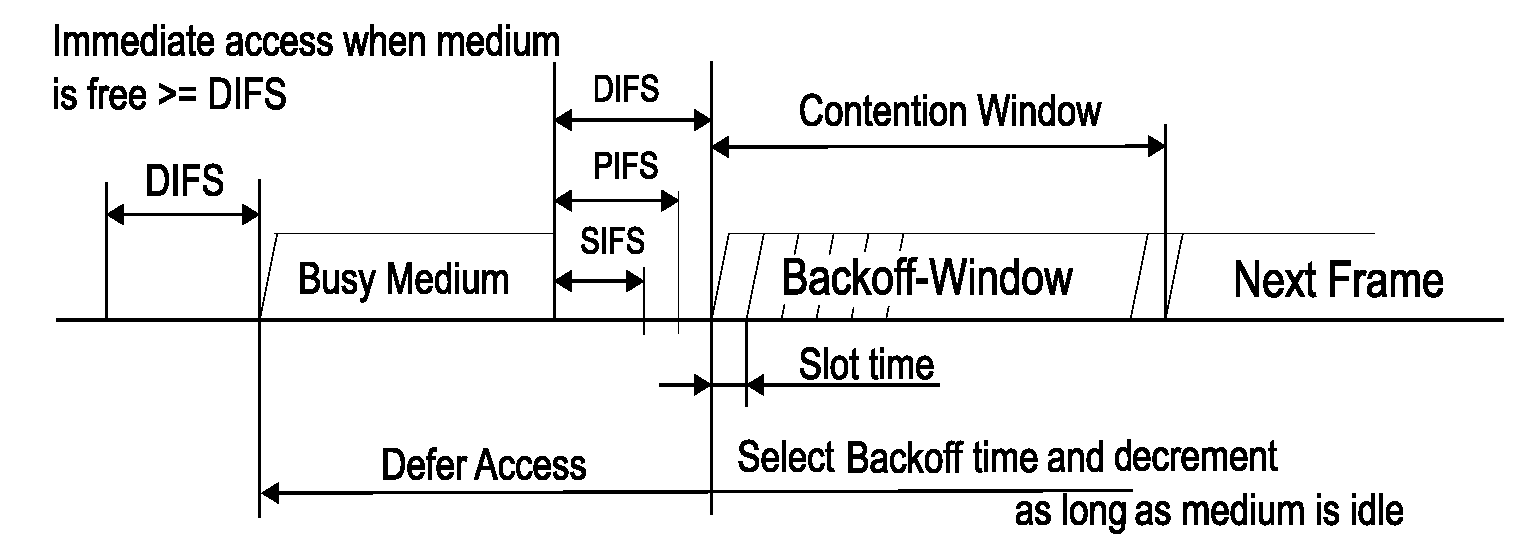
\includegraphics[width=4.5in,height=2.1in]{figures/backoff.png}
%Place caption at the bottom of the figure
\caption{IEEE 802.11 basic access method}
\label{figure:basicaccess}
\end{figure}
IEEE 802.11 basic access scheme operates in the following way: A node that wants to transmit packets listens to the medium for any transmission. If the medium is idle for a distributed inter-frame space (DIFS) duration, then the node transmits the packet. 
If the medium is busy, the node uniformly chooses a backoff value in the range (0, CW-1), where CW is the contention window, and waits for a backoff value 
%%??? 
times slot time (20 $\mu$s) by counting down to zero. The contention window (CW) is initialized to $CW_{min}$, which is dependent on the physical (PHY) layer and its default value is 31. 
Backoff counting occurs only when the medium is idle, i.e., when there are no transmissions in the network. If the medium is busy, the backoff timer is frozen and resumes when the medium becomes idle. 
If a collision occurs during transmission, the node doubles its contention window and uniformly chooses a value from the new contention window. 
The process of counting down to zero and doubling the contention window repeats until the packet is transmitted. The maximum value of the contention window is $CW_{max}$, and its default value is 1023.
\\
\indent In addition to the basic access method, an optional request to send - clear to send (RTS-CTS) mechanism is also defined by the standard. In basic access scheme, when large size frames are transmitted, the probability of collision increases. The RTS-CTS scheme is aimed at reducing the collision of large frames. In RTS-CTS scheme, the sending node first transmits a small RTS frame addressed to the receiving node. The receiving node detects the RTS frame and responds with a CTS frame after short inter-frame space (SIFS) duration. The sending node, after receiving the CTS frame, transmits the large data frame. The RTS and CTS frames exchanged by the sending and receiving nodes contain information about the length of the packet to be transmitted. The RTS and CTS frames are received by the neighboring nodes as well and based on the length of the packet to be transmitted, the neighboring nodes update their network allocation vector (NAV). The NAV value indicates the period of time during which the medium will be busy and the nodes refrain from transmitting. RTS-CTS mechanism is considered for this thesis.
\subsection{MAC Layer Misbehavior}
\label{subsection:maclayermisbehavior}
\indent The IEEE 802.11 BEB algorithm provides nodes fair access to the medium. 
Greedy nodes deviate from the standard BEB to gain more frequent access to the medium, thereby gaining more throughput from the network. 
This greedy behavior is called a MAC misbehavior, and these nodes are referred to as \textbf{misbehaving nodes}. 
Nodes that follow the standard BEB are referred to as \textbf{genuine nodes}. 
Deviating from the standard BEB is not the only way to misbehave. Nodes can modify MAC parameters such as short inter-frame space (SIFS) and DIFS, and nodes can choose values smaller than those specified in the standard. 
Giri and Jaggi 
[2]
%\cite{giriclassification} 
classify different types of misbehavior and study their effectiveness. 
Two types of misbehaviors, which they define in 
[2]
%\cite{giriclassification}
, are used in this thesis: $\alpha$-misbehavior and $CW_{fix}$-misbehavior.
\begin {itemize}
\item{{$\alpha$-misbehavior} :
Instead of choosing the backoff $b$ uniformly at random from the interval $[0 \ldots CW - 1]$, the selfish node chooses $b$ uniformly at random from the interval $[0 \ldots \alpha (CW - 1)]$, where $0 < \alpha < 1$.
Thus, the node ends up choosing a smaller backoff interval than it is supposed to and increasing its chances of accessing the channel next.
}
\item{ {Fixed contention window ($CW_{fix}$)-misbehavior}:
The selfish node sets its contention window to a small, fixed size $CW_{fix}$ and always chooses its backoff interval uniformly at random
from the interval $[0 \ldots CW_{fix}]$. 
}
\end{itemize}
According to Giri and Jaggi 
[2]
%\cite{giriclassification}
, effectiveness is defined as the percentage of improvement in throughput when a node misbehaves. This definition of effectiveness is followed in this thesis, where misbehaving nodes are considered to misbehave according to $\alpha$-misbehavior with $\alpha$ = 0.1.  
\subsection{Contribution of This Thesis}
\indent In this thesis, a new detection scheme using the inter-packet transmission (IPT) time and a collective reaction strategy are proposed. The contributions of this thesis can be summarized as follows:
\begin{itemize}
\item A method to calculate the inter-packet transmission time of a node and its neighbors is presented.
\item A detection threshold is calculated for a varying number of nodes based on the ratio of a node's own IPT time and its neighbor's IPT time. 
\item A detection rule based on the inter-packet transmission time and the detection threshold is proposed.
\item A collective reaction strategy based on the level of misbehavior in the network is proposed.
%Once misbehavior is detected, genuine nodes react by misbehaving themselves, i.e., the genuine nodes deviate from the protocol standard as well in order to react towards the misbehavior. Genuine nodes misbehave based on the level of misbehavior present in the network
\item Results from the Network Simulator-2 (NS-2) simulations are used to evaluate the proposed detection and reaction schemes. Fairness among the reacting genuine nodes is also studied.
\item Simulations results indicate that the proposed detection and reaction schemes are effective and performs well with varying number of nodes genuine and misbehaving nodes in the network. 
\item Genuine nodes, after detecting misbehavior and reacting, is able to improve its throughput and the due to the genuine  reaction, the misbehaving nodes suffer throughput loss.
\end{itemize}
\subsection{Thesis Organization}
\indent The remainder of this thesis is organized as follows: Chapter \ref{chapter:relatedwork} presents a literary overview of the work done in this area of research. Chapter \ref{chapter:detection} discusses the proposed detection mechanism. Chapter \ref{chapter:reaction} talks about the proposed misbehavior reaction strategy and derives an equation used by the reacting genuine nodes. Chapter \ref{chapter:simulation} presents the NS-2 results of the detection and reaction mechanisms discussed. Finally, Chapter \ref{chapter:conclusion} summarizes the thesis, and discusses conclusions and future directions.
\newpage
%============================================================================================================
%CHAPTER 2: RELATEDWORK
% RESET FIGURE AND TABLE COUNTER SO ANY FIGURES WILL START BEING NUMBERED AS 5.1 
% Use author name in addition to citing them. For example instead of saying "[1] observes", say "author [1] observe" 
\setcounter{table}{0}
\setcounter{figure}{0}
\setcounter{subsection}{0}
\begin{singlespace}
\begin{center}
CHAPTER 2
\section*{RELATED WORK}
\addtocounter{section}{1}
\label{chapter:relatedwork}
\end{center}
\end{singlespace}
\addtocontents{toc}{\protect\mbox{}\protect}
%\subsection{Previous Work}
\indent Much research in wireless ad hoc networks has focused on MAC-layer misbehavior. The literature related to MAC misbehavior is presented here.
\subsection{Misbehavior Detection}
\indent Radosavac et al. 
[3] 
%\cite{radosavacsprt} 
observe neighboring nodes' backoff intervals and apply the sequential probability ratio test (SPRT) on the backoff values to detect misbehavior. 
Rong et al. 
[4]
%\cite{rong} 
also use the SPRT on packet inter-arrival times and throughput degradation to detect misbehavior.
\\
\indent Raya et al. in 
[5] 
%\cite{domino} 
propose a mechanism, named DOMINO, which is deployed in access points, to detect misbehavior. This mechanism uses a modular architecture that consists of individual tests and a decision-making component (DMC). Tests are run on parameters such as shorter than DIFS, oversized network allocation vector (NAV), backoff, and scrambled frames. Each test consists of a deviation estimation component (DEC) and anomaly detection component (ADC). The test results are given as input to the decision-making component where results are aggregated using functions and weighted results are generated. This result is used in the decision of misbehavior detection.
\subsection{Reaction Mechanism}
\indent Kyasanur and Vaidya 
[6] 
%\cite{kyasanur} 
present modifications to the IEEE 802.11 protocol to detect misbehavior and to penalize selfish misbehavior. They introduce the concept of receiver-assigned backoff to detect misbehavior. The receiver sends a new backoff value to the sender in its clear to send (CTS) or acknowledgement (ACK) frame which the sender uses in its next transmission. By listening to the frames of the sender and based on its backoff values, the receiver classifies a sending node as misbehaving or genuine. The penalty scheme developed by the authors penalizes deviating hosts by assigning larger backoff values to them than those assigned to well-behaved hosts.
\\
\indent Guang et al. 
[7] 
%\cite{dream} 
propose a detection and reaction scheme for a new class of malicious misbehaviors. This proposed scheme, named DREAM (a system for detection and reaction to a timeout MAC-layer misbehavior), tackles the problem of transmission timeouts of MAC frames. The DREAM system uses two stages to detect and react to misbehavior. In the first stage, a bad credit value of a node is used in the detection. If the credit crosses a threshold, then the corresponding node is declared as a suspect node (SN). In the second stage, the SN is assigned a trust level, which is increased or decreased based on misbehavior. If the SN node misbehaves, the trust level is reduced and if the trust level falls below a threshold, the node is declared as untrusted node (UN). The trust level is propagated to the upper layers and prevents traffic via the UNs.
\\
\indent Cardenas et al. 
[8] 
%\cite{cardenas} 
compare the two popular detection algorithms SPRT 
[3] 
%\cite{radosavacsprt} 
and DOMINO 
[5] 
%\cite{domino} 
, both theoretically and by using simulations.
Guang et al. 
[9] 
%\cite{prb} 
propose modifications to the BEB algorithm in order to facilitate easy detection and penalization of a misbehaving sender. These authors propose a predictable random backoff algorithm to detect misbehavior in the network.
\\
\indent Jaggi et al. 
[10] 
%\cite{giridistributed} 
use throughput degradation to detect misbehavior. They propose two reaction methods that follow a collective misbehavior strategy. In the non-adaptive reaction scheme, all genuine nodes, upon detection of misbehavior, use a constant contention window size that is not varied. In the adaptive reaction scheme, the contention window size of the genuine nodes are dynamically computed based on the throughput degradation experienced by the individual nodes. Both strategies are distributed in nature and rely upon local information available to the genuine nodes.
\subsection{Motivation}
\indent Most of the MAC-layer misbehavior research consider access point based wireless network where misbehavior detection and reaction happen in the access points. This thesis aims to propose a detection and reaction scheme that can applied to ad hoc networks as well. 
The detection schemes proposed in other misbehavior research consider some known type of misbehavior. This thesis, does not consider specific type of misbehavior but aims to address any type of misbehavior. 
An important goal of this thesis is to propose a new parameter or criteria for misbehavior detection. Hence a new method using inter-packet transmission (IPT) time for detection of misbehavior is proposed in this thesis.
The collective reaction strategy proposed by Jaggi et al 
[10] 
%\cite{giridistributed} 
evaluate their scheme only for fixed number nodes genuine and misbehaving nodes. A good detection and reaction scheme should work irrespective the number of nodes in the networks. The detection and reaction schemes proposed in this thesis are aimed to work for varying number of nodes in the network.
\newpage
%============================================================================================================
%CHAPTER 3: DETECTION
% RESET FIGURE AND TABLE COUNTER SO ANY FIGURES WILL START BEING NUMBERED AS 5.1 
\setcounter{figure}{0}
\setcounter{table}{0}
\setcounter{subsection}{0}
\begin{singlespace}
\begin{center}
CHAPTER 3
\section*{DETECTION SCHEME}
\addtocounter{section}{1}
\label{chapter:detection}
\end{center}
\end{singlespace}
\addtocontents{toc}{\protect\mbox{}\protect}
\subsection{Introduction}
\indent This chapter discusses the proposed misbehavior detection scheme, which is based on estimating the average inter-packet transmission times of neighboring nodes and comparing them with the node's own average IPT time. This scheme has many advantages over existing schemes, which are discussed in detail here.
\subsection{Estimating Inter-Packet Transmission Time}
\indent The IPT time is defined as the time between two successful transmissions of data (DATA) packets (under the basic access mechanism) or request to send (RTS) packets (under the RTS-CTS mechanism). The following sections describe a node's own IPT time calculation and its neighbor's IPT time calculation.
\subsubsection{Node's Own IPT Time}
\indent As mentioned earlier, the IPT time is the time between transmissions of DATA packets or RTS packets. The individual or instantaneous IPT time values observed by a node are varying and random due to the binary exponential backoff algorithm. Therefore, individual IPT time values do not help in detecting misbehavior. Hence, a simple moving average of the IPT time is maintained. A simple running average is not chosen to calculate the IPT time but rather a simple moving average is used and it assists in discarding older IPT time values and considering newer IPT time values. Thus, using simple moving average to calculate IPT time reflects the current state of nodes in the network (genuine/misbehaving).
\\
\indent For a node's own IPT time calculation, the time between CTS packets is used. Even though this differs from the definition of IPT time, an IPT time calculation using CTS packets yields the correct result. This will be explained later in this section. 
\\
\indent Calculation of IPT time is as follows: When a CTS packet is successfully received, the current time is noted. When the next CTS packet is received, the previously noted time is subtracted from the current time. The subtracted value is the recent IPT time and is added with the running sum of previously calculated IPT time values. When the new IPT time is added to the running sum, the oldest IPT time is subtracted from the running sum (according to definition of simple moving average). The number of IPT time values added is 250, and the sum is divided by 250 to obtain the node's own average IPT time. This simple moving average IPT time is used in misbehavior detection. The node's own IPT time calculation is shown in Figure \ref{figure:ownipt}. 
\begin{figure}[H]
\centering
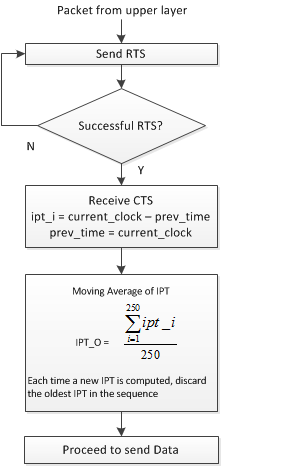
\includegraphics[width=3in,height=3.5in]{figures/ownipt.png}
\caption{Node's Own IPT time calculation}
\label{figure:ownipt}
\end{figure}
\indent According to the definition, the IPT time is the time between two RTS packets. 
In NS-2, calculating the time between two RTS packets is difficult since it involves adjusting for the retransmission of RTS packets. Hence, the time between the two CTS packets, instead of the RTS packets, is used in the IPT time calculation. In spite of the difference between the definition of IPT time and the implementation of IPT time, the value calculated by the using the CTS packets results in an accurate calculation of the IPT time. This is verified using NS-2 simulation, whereby packets are sent at a slow rate (1 packet per second), and the node's own IPT time is verified to be closer to 1 (0.999) which is same as the transmission rate (1 packet per second). 
\subsubsection{Neighbor's IPT Time Calculation}
\indent Like the node's own IPT time, each node maintains a list of neighboring nodes, and for each of the nodes, a simple moving average of the IPT time is maintained. This calculation is shown in Figure \ref{figure:neighboript}.
\begin{figure}[H]
\centering
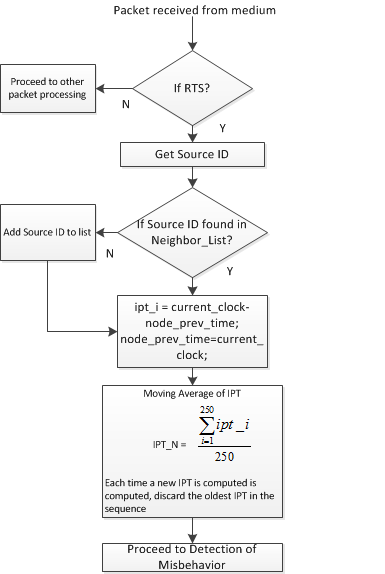
\includegraphics[width=3.3in,height=4in]{figures/neighboript.png}
\caption{Neighbor's IPT time calculation}
\label{figure:neighboript}
\end{figure}
The neighbor's IPT time is estimated by listening to the medium and calculating the time between RTS packets. A linked-list data structure is used in the neighbor's IPT time calculation and maintainence. The linked-list is indexed using node IDs. Each node in the network maintains the linked-list, and each node in the linked-list contains the neighbor's node ID and the moving average of IPT corresponding to the node. The neighbor's IPT time for a node is calculated based on the time between reception of two RTS packets from the same node. Similar to the node's own IPT time calculation, simple moving average of the IPT time values for each of the neighboring nodes is maintained. 
\\
\indent Both IPT times (a node's own IPT time and a neighbor's IPT time) are simple moving averages of individual or instantenous IPT times. The moving average is calculated over a period of 250 packets. The value of 250 is chosen for the moving average period after several trials with larger and smaller values. If the moving average period value is large, say 1000, then the node takes more time to detect misbehavior, and if the period is very small, then the node may falsely conclude misbehavior even for small variations in the network. Therefore, a value of 250 is chosen.
\begin{table}[H]
\caption{Node Parameters}
\label{table:nodeparameters}
\begin{center}
\begin{tabular}{l c}
\hline
\hline
MAC & 802.11b\\
Data Rate & 2 Mbps\\
RTS Threshold & 128 bytes\\
$CW_{Min}$ & 31\\
$CW_{Max}$ & 1023\\
Slot Time & 20 $\mu$s\\
SIFS & 10 $\mu$s\\
\hline
\end{tabular}
\end{center}
\end{table}
\indent Note that in a node's own IPT time calculation, we used the time difference between two successfully received CTS frames. But for neighbor's IPT time calculation, successful reception of RTS frames is only considered. This may lead to the conclusion that there could be a difference in number of IPT time data counts among the sending and receiving nodes due to collision of CTS frames. But this scenario does not cause any problem to the IPT time calculation. In the scenario considered for this thesis, once a successful reception of RTS is confirmed, it is guaranteed that the corresponding CTS frame will be received by the sending node since no new node in the network may suddenly appear that may cause collision of CTS frames. Moreover, in the simulation, nodes are stationary and this will not cause any loss of CTS or any other packet due to change in physical characteristics of the medium. Hence using CTS frames for own IPT time calculation and RTS frames for neighbor IPT time calculation will not cause any difference in IPT time count. 
\subsection{Simulation Details}
\label{subsection:simulationdetails}
\indent NS-2 simulation is used in finding the detection threshold discussed in the following Section \ref{subsection:detectionscheme}.
NS-2 version 2.34 is used in the evaluation of the detection and reaction schemes.
The topology consists of varying the number of sending nodes and using one receiving node. The number of sending nodes is varied with the values of 4, 9, 14 and 19. The topology is set in an area of 100x100m. 
Sending nodes transmit 512 bytes of user datagram protocol (UDP) packets at a constant bit rate of 100 packets per second. The simulation is run for 6,000 seconds.
When a node is configured as a misbehaving node, it follows $\alpha$-misbehavior with $\alpha = 0.1$. The misbehaving node(s) misbehave(s) for the entire duration of the simulation. The node parameters are captured in Table  \ref{table:nodeparameters}.
\subsection{Proposed Detection Scheme}
\label{subsection:detectionscheme}
\indent In the detection scheme proposed, the presence of misbehavior in an ad hoc network is detected using IPT time.
As mentioned earlier, each node maintains its own IPT time ($IPT_O$) and a list of neighbors' IPT times ($(IPT_N)^i$). In addition to neighbors' IPT times, a ratio of a node's own IPT time and each of its neighbor's IPT time is also maintained and it is shown in equation (\ref{equation:iptratio}).
\begin{equation}
\label{equation:iptratio}
Ratio\ of\ IPT\ time\ for\ a\ neighbor\ i,\ R_i = \frac{IPT_O}{(IPT_N)^i}
\end{equation}
Equation (\ref{equation:iptratio}) is used in the detection of misbehavior.
To define a misbehavior detection rule, a parameter called detection threshold is introduced. The misbehavior detection threshold of a node is the maximum value of the ratio in equation (\ref{equation:iptratio}) for a given number of nodes in the network. To find the threshold value, NS-2 simulations are performed when no misbehavior is present in the network. During the simulation, with four sending nodes (nodes 1, 2, 3 and 4) and a receiving node (node 5), the highest value of the ratio of IPT times for node number 1 is noted. The simulation is repeated with 9, 14 and 19 sending nodes. This is captured in Figure \ref{figure:worstcaseratio} which represents the worst case $\frac{IPT_O}{(IPT_N)^i}$ when no misbehavior is present in network. 
\begin{figure}[H]
\centering
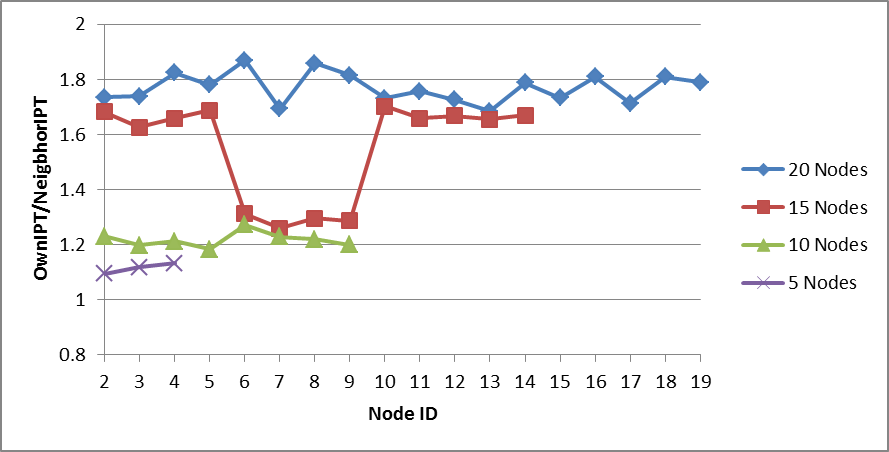
\includegraphics[width=3.2in,height=2.2in]{figures/worstcaseratio.png}
\caption{Worst case ratio of node's own IPT time to neighbor's IPT time (presence of misbehavior)}
\label{figure:worstcaseratio}
\end{figure}
If this ratio exceeds the detection threshold, then the node concludes presence of misbehavior in the network.
\indent The average values of the worst case scenario for different network sizes are captured in Table \ref{table:averageworstcase}. 
\begin{table}[H]
\caption{Average of Worst Case IPT Time Ratios}
\label{table:averageworstcase}
\begin{center}
\begin{tabular}{l c}
\hline
\hline
Nodes & IPT Time Ratio\\
5 & 1.15\\
10 & 1.25\\
15 & 1.55\\
20 & 1.75\\
\hline
\end{tabular}
\end{center}
\end{table}
An example of a detection threshold for ten nodes is discussed here.
Based on the value in Table \ref{table:averageworstcase}, the detection threshold of 1.25 is chosen for ten nodes, i.e., if $\frac{IPT_O}{(IPT_N)^i}$ exceeds 1.25, then the corresponding neighbor is declared as misbehaving. Similar approach can be used to set appropriate thresholds for N = {5,15,20} nodes as well. This ratio is also used during the reaction mechanism. The reaction mechanism is discussed in detail in the Chapter \ref{chapter:reaction}.
\indent The inverse of $\frac{IPT_O}{(IPT_N)^i}$ is the misbehavior strength ($\gamma$), and it lies between 0 and 1. More precisely, $0 < \frac{1}{\frac{IPT_O}{(IPT_N)^i}} \leq 1$. In the case of ten nodes, if $\frac{IPT_O}{(IPT_N)^i}$ is found to be 3.5, then the misbehavior strength is $0.28$.
\begin{algorithm}
\caption{Detection Algorithm}
\label{algorithm:detection}
\begin{algorithmic}
\STATE Input: $IPT_O\ and\ (IPT_N)^i$
\STATE m=0
\STATE i=1
\WHILE{$i<=N$}
    \IF {$\frac{IPT_O}{(IPT_N)^i} > (1.25)$} 
        \STATE $mark\ node\ as\ misbehaving$
        \IF {$m\ <\ \frac{IPT_O}{(IPT_N)^i}\ ratio$}
        	\STATE $m = \frac{IPT_O}{(IPT_N)^i}$
        \ENDIF
	\ENDIF
	\STATE $i++$
\ENDWHILE

\IF {$m\ >\ 1$}
	\STATE $m = \frac{1}{\frac{IPT_O}{(IPT_N)^i}}$
	\RETURN $m$
\ELSE
	\RETURN $1$
\ENDIF
\end{algorithmic}
\end{algorithm}
This detection scheme is presented in Algorithm \ref{algorithm:detection}. The detection algorithm is run by each of the genuine nodes in the networks. Since misbehavior detection is based on the inter-packet transmission time, the detection algorithm is invoked whenever neighbor IPT time is updated, i.e., when a packet is received from a neighbor. The detection algorithm has access to both the node's own IPT time and the node's linked list, which maintains the neighbor's IPT time.
\\
\indent The detection algorithm traverses through the linked list and calculates the ratio of its own IPT time and each neighbor's IPT time. If the ratio exceeds the detection threshold, then the corresponding node is marked as misbehaving, and the variable $m$ indicating misbehavior is updated with the $\frac{IPT_O}{(IPT_N)^i}$. If more than one neighboring node is misbehaving, then the greatest $\frac{IPT_O}{(IPT_N)^i}$ is considered, and $m$ is updated with that value. The inverse of $\frac{IPT_O}{(IPT_N)^i}$ is returned by the detection algorithm as the misbehavior strength ($\gamma$) present in the network.
The detection scheme returns 1, if no misbehavior is detected.
The detection scheme is used only by genuine nodes; misbehaving nodes do not use any detection scheme.
\\
\indent The detection scheme proposed uses a new parameter namely the IPT time. This method has not been proposed by any  literature in this field of research. The results shown in Chapter \ref{chapter:simulation} indicate that scheme is successful in detecting misbehaviors. The detection scheme proposed, unlike 
[6]
%\cite{kyasanur}
, does not require any protocol modifications. The information collected the genuine nodes are local to the nodes and the detection scheme is easily scalable. An important characteristic of this detection scheme is that it is dynamic in nature and can detect if the nodes have stopped misbehaving and returned to normal BEB algorithm. 
\subsection{Summary}
\label{summarydetection}
\indent This chapter explains the estimation of a node's own IPT time and also its neighbor's IPT times. It also discusses the choice of detection threshold and how it varies with the number of nodes. A detection scheme based on the ratio of a node's own IPT time and neighbor's IPT time is presented.
\newpage
%============================================================================================================
%CHAPTER 4: REACTION
% RESET FIGURE AND TABLE COUNTER SO ANY FIGURES WILL START BEING NUMBERED AS 5.1 
\setcounter{figure}{0}
\setcounter{table}{0}
\setcounter{subsection}{0}
\begin{singlespace}
\begin{center}
CHAPTER 4
\section*{REACTION SCHEME}
\addtocounter{section}{1}
\label{chapter:reaction}
\end{center}
\end{singlespace}
\addtocontents{toc}{\protect\mbox{}\protect}
\subsection{Introduction}
\indent The reaction scheme is the strategy or methodology used by the genuine nodes to react against misbehavior in order to improve its own throughput and to penalize the misbehaving node(s). This chapter describes the design of the proposed reaction strategy used by the genuine nodes. $CW_{fix}$-misbehavior, defined in Section \ref{subsection:maclayermisbehavior}, is used by the genuine nodes for a reaction scheme. An equation to compute an appropriate value to use for $CW_{fix}$ is also presented in this chapter.
\subsection{Desired Properties of Reaction Scheme}
\label{subsection:propertiesofreaction}
\indent The reaction scheme employed by the genuine nodes should be simple and distributed, and should result in minimal or no protocol change. 
Jaggi et al. 
[10] 
%\cite{giridistributed} 
used a collective misbehavior reaction strategy. This thesis also uses, a collective misbehavior reaction strategy.
In a collective reaction strategy, when the genuine nodes detect misbehavior in the network, they also start misbehaving to improve their throughput. All genuine nodes follow the same reaction scheme.
The collective reaction strategy used here is distributed and requires minimal protocol modification.\\
\indent The reaction scheme proposed uses a fixed contention window ($CW_{fix}$) type of misbehavior. Genuine nodes choose a random backoff from this fixed contention window and do not double the contention window as in normal operation of the IEEE 802.11 BEB algorithm. The value of the $CW_{fix}$ used by the genuine nodes should be smaller (nodes back off for a smaller duration) in order to provide an advantage to the genuine nodes, i.e., more frequent access to the medium. If the $CW_{fix}$ is too small, then genuine nodes will spend most of the time in collision and less time in successful transmission of packets. Thus, a tradeoff is involved in the choice of the $CW_{fix}$ value. Also if the misbehavior is mild a larger $CW_{fix}$ may suffice but if the misbehavior is severe a smaller $CW_{fix}$ might be needed. This tradeoff and a proposed scheme to compute an effective value for $CW_{fix}$ are discussed here.
\subsection{Design of Reaction Scheme} 
\label{subsection:reactiondesign} 
\indent Three parameters are used in the reaction scheme:
\begin{itemize}
\item Reaction Type - The type of misbehavior used by the genuine nodes to react against misbehavior.
\item Reaction Factor - The strength of misbehavior used by the genuine nodes. In the case of the $CW_{fix}$-misbehavior type, the reaction factor is $CW_{fix}$. If $\alpha$-misbehavior is used for the reaction, then the reaction factor is $\alpha$.
\item Reaction Count - This count is used to compensate for the time spent until misbehavior is detected. Note that genuine nodes do not react until misbehavior is detected. This count is incremented when misbehavior is detected and decremented when no misbehavior is detected. If reaction count is greater than zero, reaction is applied. If the count is zero and no misbehavior is detected, then the genuine nodes do not react. 
\end{itemize}
Misbehavior is detected as described in Chapter \ref{chapter:detection}. The detection scheme returns the presence of misbehavior in the network. If misbehavior is present, then the strength of misbehavior ($\gamma$) is returned. This is used in calculating the reaction factor.
As discussed in the previous section, the reaction scheme used in the experiments conducted in this thesis is $CW_{fix}$ misbehavior. Hence, the reaction factor mentioned earlier is $CW_{fix}$. Note that other reaction schemes are equally suitable and could also be used. The $CW_{fix}$ used by reacting genuine nodes should address the tradeoff, discussed earlier in Section \ref{subsection:propertiesofreaction}, about achieving the maximum gain while minimizing collisions in the network. If $CW_{fix}$ is smaller for a large number of nodes, then the number of collisions will increase, thus leading to less throughput. Therefore, $CW_{fix}$ should be directly proportional to number of nodes in the network.
\\
\indent Bianchi et al. 
[11] 
%\cite{bianchioptimalcw} 
propose a method for increasing the network saturated throughput by using an optimal contention window instead of the IEEE802.11 BEB algorithm. It derives optimal CW equations for the basic access scheme and the RTS-CTS mechanism. By combining an optimal CW value and the misbehavior strength, $CW_{fix}$ is derived.
The $CW_{optimal}$ equation in the case of the RTS-CTS mechanism presented by Bianchi et al. 
[11] 
%\cite{bianchioptimalcw} 
is
\begin{equation}
\label{equation:cwoptimalrts}
CW_{optimal} = n * \sqrt{2K}
\end{equation}
where n is number of nodes contending for the channel, $K = T_{PH} + T_{RTS} + DIFS + \tau$, $T_{PH}$ is the PHY header transmission time, and $T_{RTS}$ is the RTS transmission time, and $\tau$ is the propagation delay. K is expressed in slot times. In this simulation, the values used are 
$T_{PH} + T_{RTS} = 352 \mu s$, 
$DIFS = 50 \mu s$, 
$\tau = 2 \mu s$ and  
$2K = 6.356099$.
\\
Using equation (\ref{equation:cwoptimalrts}), the $CW_{optimal}$ values for different number of nodes are presented in Table \ref{table:optimalcw}.
\begin{table}[H]
\caption{Optimal CW}
\label{table:optimalcw}
\begin{center}
\begin{tabular}{l c}
\hline
\hline
Nodes & Contention Window\\
5 & 25\\
10 & 57\\
15 & 89\\
20 & 121\\
\hline
\end{tabular}
\end{center}
\end{table}
As discussed earlier, the detection scheme returns the strength of the misbehavior present in the network. This value is actually the ratio of the neighbor's IPT time and the node's own IPT time. 
Various values of $CW_{fix}$ for the reaction is tried to see which value performs the best. The best value found using experimentation for different number of nodes is shown in Table \ref{table:desiredcwfix}.
The objective of the reaction scheme is to express and compute the desired best $CW_{fix}$ value in terms of known and computed system parameters such as number of nodes (N), $CW_{optimal}$ and misbehavior strength ($\gamma$), as returned by detection algorithm.
%To provide a good reaction, genuine nodes should react with $CW_{fix}$ values, as described in Table \ref{table:desiredcwfix}. 
%These values are found by experimenting with different values of $CW_{fix}$.
%Expressing $CW_{fix}$ in terms of $CW_{optimal}$ and $\frac{IPT_O}{(IPT_N)^i}$ alone does not produce the $CW_{fix}$ values presented in Table \ref{table:desiredcwfix}. 
\begin{table}[H]
\caption{Desired $CW_{fix}$}
\label{table:desiredcwfix}
\begin{center}
\begin{tabular}{l c}
\hline
\hline
Nodes & Best value of $CW_{fix}$ for reaction\\
5 & 2\\
10 & 4\\
15 & 6\\
20 & 8\\
\hline
\end{tabular}
\end{center}
\end{table}
%Therefore, another parameter, number of nodes in the network, is also included. The square of the number of nodes is used to achieve the desired $CW_{fix}$ values. Since we have a squared number, the $CW_{fix}$ values will be large and will not result in strong reaction. Hence, to reduce the $CW_{fix}$ values, a small constant of 0.005 is multiplied with $CW_{fix}$.
%\\
\indent Using the $CW_{optimal}$ and misbehavior strength ($\gamma$), and the number of nodes, equation (\ref{equation:cwfix}) is proposed to calculate the $CW_{fix}$ which is used by the reacting genuine nodes. Let $N_{c}$ denote the neighbor node count.
\begin{equation}
\label{equation:cwfix}
CW_{fix} = CW_{optimal} * (N_{c})^2 * (\gamma)^2 * 0.005
\end{equation}
Note that this value may change for every RTS packet received by the node. According to equation (\ref{equation:cwfix}), $CW_{fix}$ increases as the number of nodes increases as described in Section \ref{subsection:reactiondesign}. Also $CW_{fix}$ decreases if misbehavior strength increases (i.e., $\gamma$ decreases).
\\
\indent The reaction scheme used by the genuine nodes is presented in Algorithm \ref{algorithm:reaction}. This algorithm uses misbehavior strength ($\gamma$) as the input. This is returned by the detection rule described in Algorithm \ref{algorithm:detection}. 
The aim of the reaction algorithm is to set the parameters $misbhType$ and $misbhValue$ to zero (if no misbehavior is present) and to an appropriate value (if misbehavior is detected).
In Algorithm \ref{algorithm:reaction}, $misbhType$ is $CW_{fix}$-misbehavior.
When misbehavior is detected ($\gamma < 1$), $misbhValue$ takes the value calculated according to equation (\ref{equation:cwfix}). 
\begin{algorithm}[t]
\caption{Reaction Scheme}
\label{algorithm:reaction}
\begin{algorithmic}
\STATE Input: $\gamma$
\IF {$\gamma < $ 1}
	\STATE $CW_{fix}\ =\ CW_{optimal}\ *\ (N_{c})^2\ *\ (\gamma)^2\ *\ 0.005$
	\STATE $CW_{fix}\ =\ (CW_{fix}\ >\ 3)\ ?\ CW_{fix}\ :\ 3$
	\STATE \COMMENT {Presence of Misbehavior and reacting}
	\STATE $misbhReactCount\ =\ misbhReactCount\ +\ 2$
	\STATE $misbhType\ =\ MISBH\_REACT\_TYPE$
	\STATE \COMMENT {$MISBH\_REACT\_TYPE$ indicates $CW_{fix}$-misbehavior}
	\STATE $misbhValue\ =\ CW_{fix}$
\ELSIF {$misbhReactCount$}
	\STATE \COMMENT {No Misbehavior but reacting}
	\STATE $misbhReactCount\ =\ misbhReactCount\ -\ 1$
	\STATE $misbhType\ =\ MISBH\_REACT\_TYPE$
	\STATE $misbhValue\ =\ \frac{CW_{min}}{2}$
\ELSE
	\STATE \COMMENT {No Misbehavior and not reacting}
	\STATE $misbhType\ =\ 0$
	\STATE $misbhValue\ =\ 0$
\ENDIF
\end{algorithmic}
\end{algorithm}
%As previously mentioned, the reaction scheme also uses a counter called $misbhReactCount$. 
\\
\indent Genuine nodes react, i.e., misbehave only after misbehavior has occurred in the network. 
This may take some time to get reflected in the simple moving average of the IPT calculation discussed in Chapter \ref{chapter:detection}. 
To compensate for the misbehavior that has already occurred, genuine nodes continue to react even after detecting that no misbehavior is present in the network. 
This is accomplished by maintaining a counter $misbhReactCount$. This counter is incremented (by two) when the node has detected misbehavior (and nodes are reacting) and it is decremented (by one) when there is no misbehavior but continue to react until $misbhReactCount$ reaches zero. When $misbhReactCount$ is decremented, a mild reaction is required and hence the $CW_{fix}$ used during this period is $\frac{CW_{min}}{2}$. 
When no misbehavior is detected and $misbhReactCount$ is zero, then the genuine nodes do not react and follow the IEEE 802.11 BEB algorithm.
The simulation results of the detection scheme and the reaction scheme are presented in Chapter \ref{chapter:simulation}.
\\
\indent The proposed reaction scheme uses a novel method of controlling reaction strength based on IPT time. The scheme considers factors like number of nodes in the networks, the misbehavior strength and adjusts the reaction dynamically. A distinctive feature of this scheme is that it is scalable to any network size and the scheme can be extended to other reaction types (like $\alpha$ misbehavior instead of $CW_{fix}$ misbehavior.) Scheme is adaptive as in if misbehaving nodes stops misbehaving or returns to normal behavior, the genuine nodes also return to normal BEB behavior. The reaction requires a minimal protocol modification and the decisions made by the genuine nodes are totally based on the local information available to the nodes.
\subsection{Summary}
\label{summaryreaction}
\indent This chapter presents the proposed reaction scheme used by the genuine nodes. The genuine nodes use $CW_{fix}$-misbehavior. Based on the strength of the misbehavior present and the number of nodes in the network, the reaction scheme calculates the appropriate $CW_{fix}$ values to be used by the genuine nodes. The reaction scheme dynamically adjusts according to the strength of misbehavior present in the network.
\newpage
%============================================================================================================
%CHAPTER 5: RESULTS
% RESET FIGURE AND TABLE COUNTER SO ANY FIGURES WILL START BEING NUMBERED AS 5.1 
\setcounter{figure}{0}
\setcounter{table}{0}
\setcounter{subsection}{0}
\begin{singlespace}
\begin{center}
CHAPTER 5
\section*{SIMULATION RESULTS}
\addtocounter{section}{1}
\label{chapter:simulation}
\end{center}
\end{singlespace}
\addtocontents{toc}{\protect\mbox{}\protect}
\subsection{Introduction}
\indent This chapter presents the simulation results of detection and reaction mechanisms performed using the Network Simulator-2.
Network topology, simulation parameter details, and metrics used in the experiments conducted are presented here.
Results are captured by varying number of nodes, reaction or no reaction and number of misbehaving nodes.
\subsection{NS-2 Simulator}
\indent NS-2 is used for the simulation study. This discrete event simulator is written in OTCL and C++. OTCL serves as the front end of the simulator, and actual simulation is implemented in C++. 
NS-2 is used because it is open source and free to use. Moreover, it supports a variety of protocols, and most of the wireless network research all over the world is simulated in NS-2.
Detection and reaction schemes presented in Chapters \ref{chapter:detection} and \ref{chapter:reaction} are implemented in C++ module of NS-2. C++ code modifications that are required to implement the proposed detection and reaction schemes and TCL topology script are presented in Appendices A and B respectively.
\subsection{Performance Metrics}
\indent Following are the metrics considered in this thesis:
\begin{itemize}
\item Inter-packet transmission time is used in detection of misbehavior, as described in Chapter \ref{chapter:detection}. 
It is defined as the time between two successfully transmitted data packets by a node. 
Each node maintains its own IPT time and the IPT time of its neighboring nodes.
A node listens to the medium, and based on the difference between the time of consecutive RTS arrivals, the node calculates its neighbor's IPT time. 
In addition to this, each node maintains a ratio of its own IPT time and each of its neighbor's IPT time. 
The nodes in NS-2 calculate the IPT time at the run time. 
The calculation of inter-packet transmission time is performed dynamically by the nodes and is used in misbehavior detection. 
\item Throughput is used in the evaluation of the effectiveness of detection and reaction schemes. 
Once the simulation is complete, using a PERL script, the trace output of the simulation is analyzed and throughput of nodes is computed. 
Based on the improvement of genuine nodes' throughput, it can be concluded if the detection and reaction mechanisms are effective in dealing with the presence of misbehavior in the network.
\item Fairness in throughput among nodes is also calculated. Jain's fairness index 
[12] 
%\cite{jainfairness} 
is used in the throughput fairness calculation.
\end{itemize}
\subsection{Simulation Details}
\indent The simulation details are the same as mentioned in Section \ref{subsection:simulationdetails}.
\subsection{Results}
\label{section:results}
Simulation is run by varying the following:
\begin{itemize}
\item Number of nodes in the network (5, 10, 15, 20)
\item Number of misbehaving nodes (1, 2)
\item Genuine nodes' reaction or no reaction.
\end{itemize}
The three different throughput information (in absence of misbehavior, in presence of misbehavior and when genuine nodes react) are captured in Figures \ref{figure:05nodes} to \ref{figure:20nodes}. The largest numbered node in each figure is the misbehaving node and the other nodes are the genuine nodes. The throughput values shown are the individual genuine node's throughput at the end of simulation.
Figure \ref{figure:05nodes_1misbehavior_alpha1} depicts the following:
\begin{itemize}
\item Throughput of four nodes in the absence of misbehavior
\item Throughput of four nodes when one node is misbehaving
\item Throughput of four nodes when genuine nodes react using the reaction scheme discussed in Chapter  \ref{chapter:reaction}. 
\end{itemize}
\begin{figure}[H]
\centering
\subfloat[1 misbehaving node]{
\label{figure:05nodes_1misbehavior_alpha1}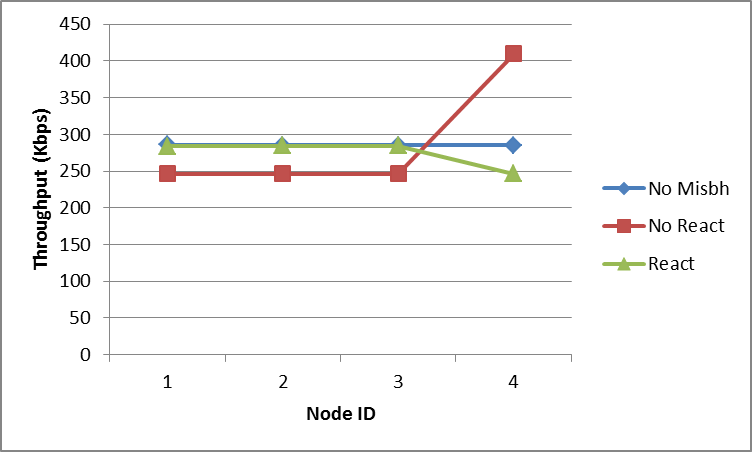
\includegraphics[width=3.2in,height=2.2in]{figures/05nodes_1misbh.png}
}
\subfloat[2 misbehaving nodes]{
\label{figure:05nodes_2misbehavior_alpha1}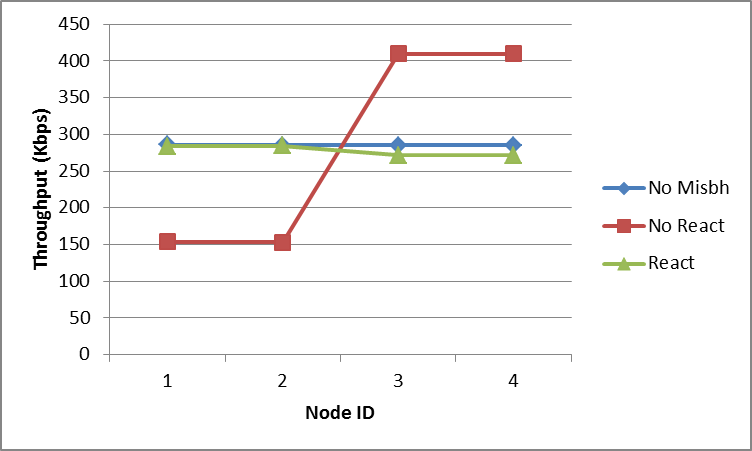
\includegraphics[width=3.2in,height=2.2in]{figures/05nodes_2misbh.png}
}
\caption{Throughput with N=5 nodes}
\label{figure:05nodes}
\end{figure}
\indent In the absence of misbehavior, the throughput of all nodes is $\approx$ 285 Kbps. It is clear from the Figures \ref{figure:05nodes_1misbehavior_alpha1} and \ref{figure:05nodes_2misbehavior_alpha1} that when the genuine nodes react in the presence of misbehavior, the throughput of the misbehaving nodes drops significantly. 
The genuine nodes' throughput, after reaction, is nearly the same ($\approx$ 284 Kbps) as the no-misbehavior scenario. 
According to the reaction scheme discussed in Section \ref{subsection:reactiondesign}, the genuine nodes, upon detecting presence of misbehavior in the network, choose a small $CW_{fix}$ value instead of following the IEEE 802.11 BEB algorithm.  Since the genuine nodes themselves misbehave, the genuine nodes see an increase in throughput because of their increased access to the medium. The $CW_{fix}$ value chosen by the genuine nodes vary dynamically throughout the simulation in accordance with the strength of misbehavior present in the network.
Similar behavior is observed when two nodes are misbehaving, as shown in Figure \ref{figure:05nodes_2misbehavior_alpha1}.
\\
\indent Figure \ref{figure:10nodes_1misbehavior_alpha1} depicts the throughput of nine nodes in the absence of misbehavior, when one node is misbehaving and the throughput increase of the genuine nodes when the genuine nodes react. 
\begin{figure}[H]
\centering
\subfloat[1 misbehaving node]{
\label{figure:10nodes_1misbehavior_alpha1}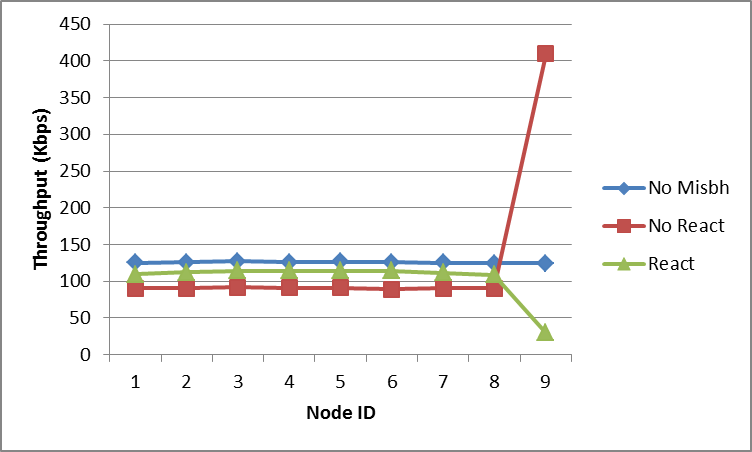
\includegraphics[width=3.2in,height=2.2in]{figures/10nodes_1misbh.png}
}
\subfloat[2 misbehaving nodes]{
\label{figure:10nodes_2misbehavior_alpha1}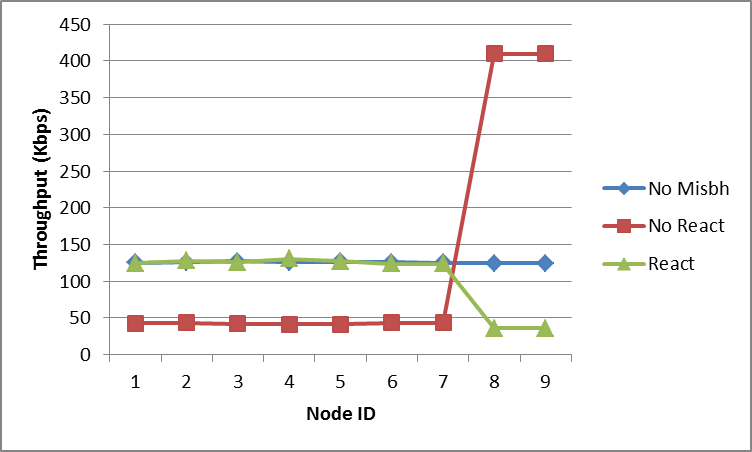
\includegraphics[width=3.2in,height=2.2in]{figures/10nodes_2misbh.png}
}
\caption{Throughput with N=10 nodes}
\label{figure:10nodes}
\end{figure}
Throughput of the nodes in the absence of misbehavior is $\approx$ 125 Kbps. Figure  \ref{figure:10nodes_1misbehavior_alpha1} shows when a node misbehaves, throughput of the genuine nodes falls by approximately $28\%$ to 90 Kbps. When the genuine nodes react, throughput of the individual genuine nodes increase by $24\%$ to 112 Kbps.
Figure \ref{figure:10nodes_2misbehavior_alpha1} depicts the scenario when two nodes are misbehaving. Due to the two misbehaving nodes, the genuine nodes suffer a greater throughput loss (dropping to 43 Kbps) and the misbehavior strength is larger i.e., $\gamma$ is smaller than in \ref{figure:10nodes_1misbehavior_alpha1}.
\begin{figure}
\centering
\subfloat[1 misbehaving node]{
\label{figure:15nodes_1misbehavior_alpha1}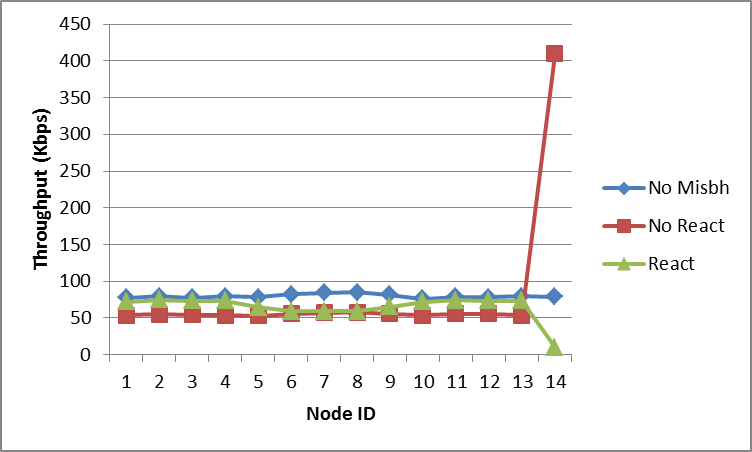
\includegraphics[width=3.2in,height=2.2in]{figures/15nodes_1misbh.png}
}
\subfloat[2 misbehaving nodes]{
\label{figure:15nodes_2misbehavior_alpha1}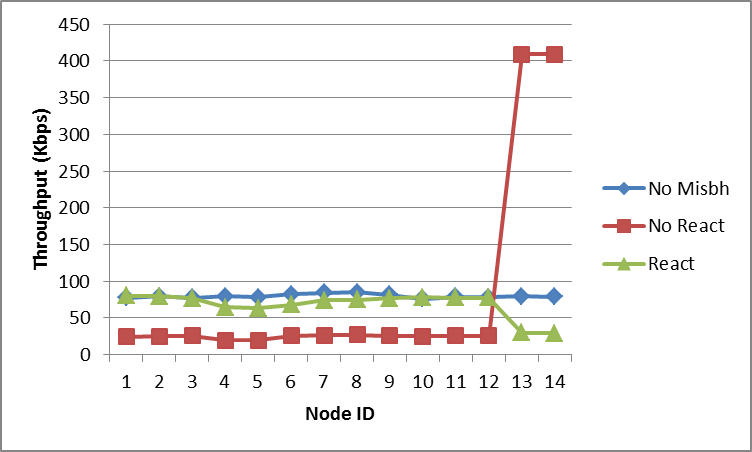
\includegraphics[width=3.2in,height=2.2in]{figures/15nodes_2misbh.png}
}
\caption{Throughput with N=15 nodes}
\label{figure:15nodes}
\end{figure}
From the perspective of the genuine nodes, the misbehavior is very strong in the network, and nodes aggressively react, resulting in an increase in throughput to levels greater than 125 Kbps.
A similar explanation holds for the 14 and 19 sending nodes, and results are depicted in Figures \ref{figure:15nodes_1misbehavior_alpha1}, \ref{figure:15nodes_2misbehavior_alpha1}, \ref{figure:20nodes_1misbehavior_alpha1}, and \ref{figure:20nodes_2misbehavior_alpha1}.
\begin{figure}
\centering
\subfloat[1 misbehaving node]{
\label{figure:20nodes_1misbehavior_alpha1}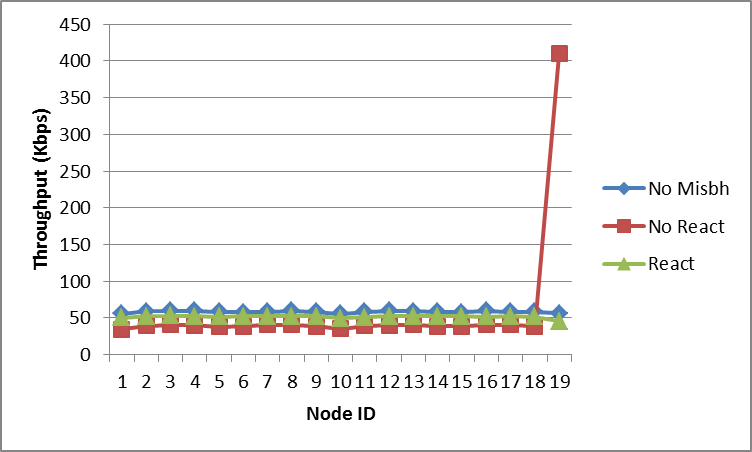
\includegraphics[width=3.2in,height=2.2in]{figures/20nodes_1misbh.png}
}
\subfloat[2 misbehaving nodes]{
\label{figure:20nodes_2misbehavior_alpha1}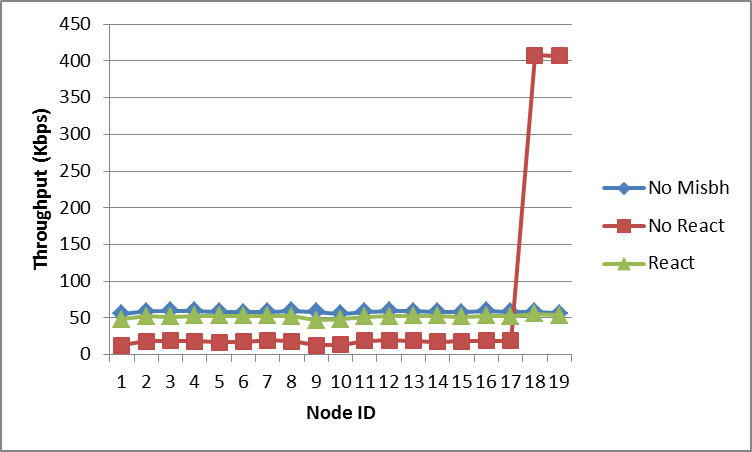
\includegraphics[width=3.2in,height=2.2in]{figures/20nodes_2misbh.png}
}
\caption{Throughput with N=20 nodes}
\label{figure:20nodes}
\end{figure}
In all of these scenarios, the fairness among the throughput achieved by genuine nodes is close to optimal and is around $0.99$ in all cases. This is depicted in the Figures \ref{figure:fairness_1misbh} and \ref{figure:fairness_2misbh}.
\begin{figure}
\centering
\subfloat[1 misbehaving node]{
\label{figure:fairness_1misbh}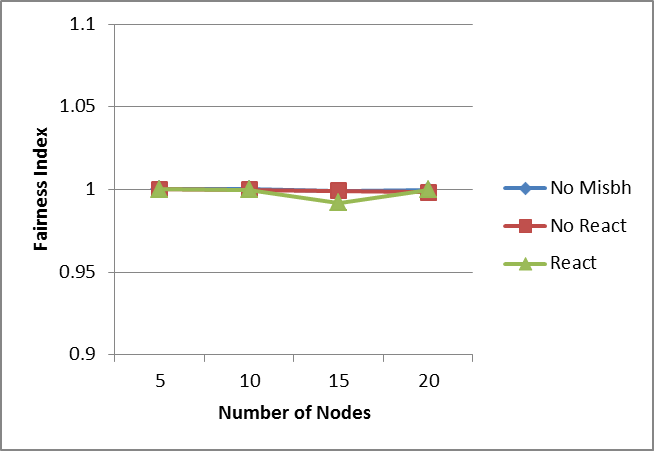
\includegraphics[width=3.2in,height=2.2in]{figures/fairness_1misbh.png}
}
\subfloat[2 misbehaving nodes]{
\label{figure:fairness_2misbh}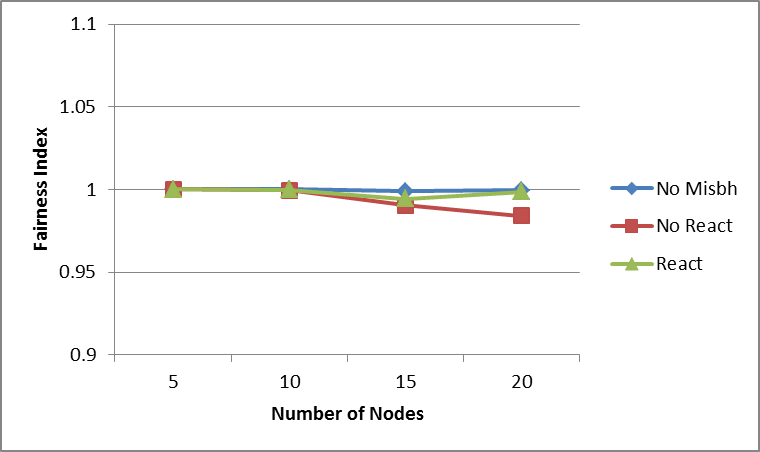
\includegraphics[width=3.2in,height=2.2in]{figures/fairness_2misbh.png}
}
\caption{Fairness among genuine nodes}
\label{figure:fairness}
\end{figure}
To measure the reaction effectiveness of the reaction scheme, a metric called reaction effectiveness is used and is defined as 
\begin{equation}
\label{equation:reaction_effectiveness}
re = \frac{genuine\ nodes'\ average\ throughput\ with\ reaction}{genuine\ nodes'\ average\ throughput\ with\ no\ misbehavior} * 100
\end{equation}
Figure \ref{figure:reaction_effectiveness} depicts the reaction effectiveness. 
Reaction effectiveness (re) values closer to $100\%$ indicate that the genuine nodes, after reaction, were able to achieve as much throughput as they would have achieved if there was no misbehavior. From the results, reaction is more effective when number of misbehaving nodes is larger and when the total number of nodes in the network is smaller. As a result of applying reaction, the overall network throughput decreases slightly. This is expected, since all the genuine nodes are misbehaving under the reaction scheme. However, most of the loss in throughput is shared by misbehaving nodes, since the misbehavior effectiveness is close to $100\%$ for many scenarios and is greater than $85\%$ in all scenarios evaluated.
\begin{figure}
\centering
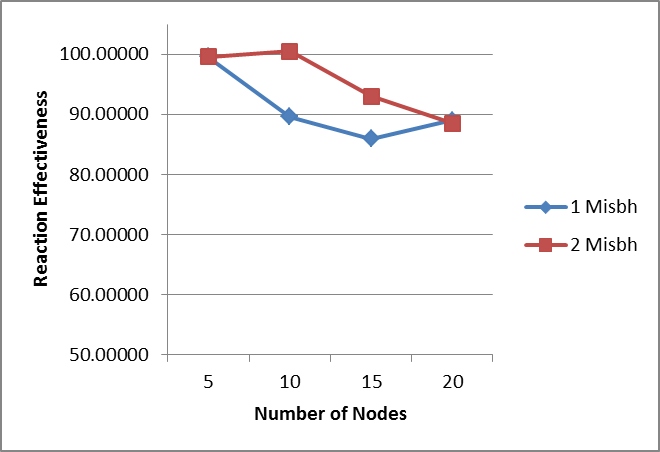
\includegraphics[width=3.2in,height=2.2in]{figures/reaction_effectiveness.png}
\caption{Reaction effectiveness}
\label{figure:reaction_effectiveness}
\end{figure}
\begin{figure}[H]
\centering
\subfloat[1 misbehaving node]{
\label{figure:network_1misbh}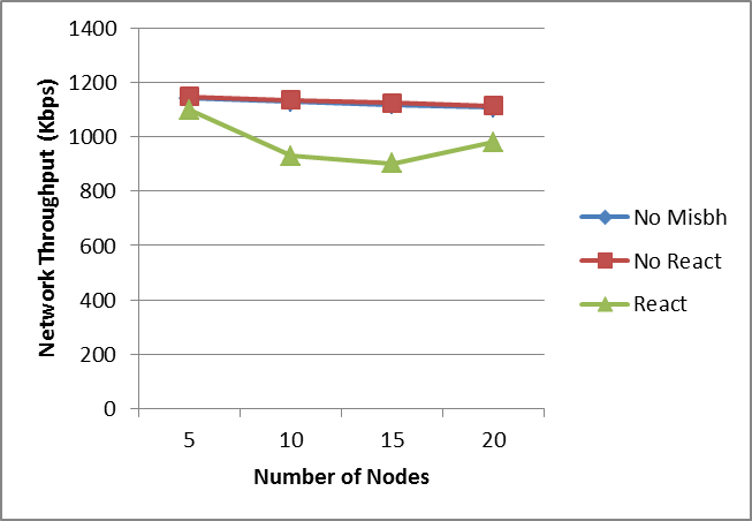
\includegraphics[width=3.2in,height=2.2in]{figures/network_1misbh.png}
}
\subfloat[2 misbehaving nodes]{
\label{figure:network_2misbh}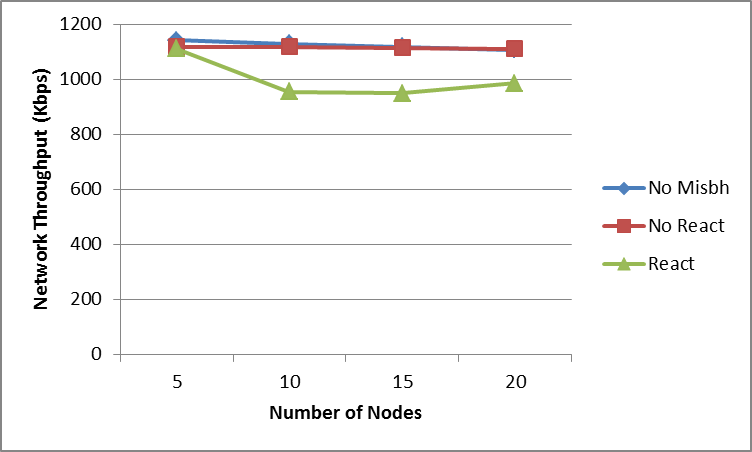
\includegraphics[width=3.2in,height=2.2in]{figures/network_2misbh.png}
}
\caption{Overall network throughput}
\label{figure:networkthroughput}
\end{figure}
\subsection{Discussion}
\label{resultdiscussion}
\indent The collective reaction strategy using the fixed contention window ($CW_{fix}$) is shown to be effective for MAC-layer misbehavior. The throughput of the genuine nodes almost reaches the original levels and fairness is also maintained among the genuine nodes. As the number of nodes become larger in the network, a drop in reaction effectiveness is observed. In this scenario of increasing number of nodes, the genuine nodes do not suffer greater throughput loss and hence do not react strongly, but reaction is strong enough to achieve throughput close to the level observed when no misbehavior is present. When genuine nodes react, that is collectively misbehave, all the nodes try to access the medium very frequently. This results in increased collision in the network and the overall network throughput drops. This side effect of the collective reaction strategy can be seen in Figures \ref{figure:network_1misbh} and \ref{figure:network_2misbh}.
\subsection{Summary}
\label{summarysimulation}
\indent This chapter analyzes the misbehavior reaction with a varying number of nodes and varying number of misbehaving nodes. 
Reaction effectiveness, throughput of nodes and fairness among the genuine nodes are also discussed. 
The effect of reaction strategy on the overall network throughput is also discussed.
\newpage
%============================================================================================================
% CHAPTER 6: CONCLUSIONS 
% RESET FIGURE AND TABLE COUNTER SO ANY FIGURES WILL START BEING NUMBERED AS 6.1 
\setcounter{figure}{0}
\setcounter{table}{0}
\setcounter{subsection}{0}
\begin{singlespace}
\begin{center}
CHAPTER 6
\section*{CONCLUSIONS AND FUTURE WORK}
\addtocounter{section}{1}
\label{chapter:conclusion}
\end{center}
\end{singlespace}
\addtocontents{toc}{\protect\mbox{}\protect}
\indent This chapter summarizes the work done in this thesis and provides conclusions of the results. Suggestions for future work are also provided.
\subsection{Summary and Contributions}
\indent In this thesis, a novel method for detecting misbehavior in a wireless ad hoc network is presented.
The inter-packet transmission times of a node and its neighbors are used to detect misbehaviors in the network. 
A collective misbehavior reaction strategy is used to suppress the misbehaving node and allow genuine nodes to regain their own throughput. 
Important characteristics of both the detection and reaction mechanisms are that they are distributed in nature and rely only on a node's local information. The detection and reaction mechanisms require minimal protocol change and thus are easily implementable in practice.
NS-2 simulations are performed to evaluate the proposed detection and reaction mechanisms. Results indicate significant improvement in throughput of the genuine nodes and reduction in the misbehaving nodes' throughput. 
Scalabity of the detection and reaction strategies are also studied, and the results indicate that detection and reaction mechanisms are effective with a varying number nodes in the network. 
\subsection{Conclusions}
\indent Detection of misbehavior based on the ratio of inter-packet transmission is very effective, and the detection threshold is designed to vary with the number of nodes in the network.
The proposed collective reaction strategy is effective in restoring the node's original throughput and in penalizing the misbehaving node.
The distributed nature of the reaction scheme facilitates the genuine nodes' local decision making capability and eliminating the need for central authority to monitor the network and penalize the misbehaving nodes. 
During reaction, the fairness among the throughput achieved by genuine nodes is close to optimal and is around $0.99$ in all cases. 
%The reaction scheme is very effective when there are large number of nodes and when there are more misbehaving nodes in the network.
As expected, due to collective misbehavior strategy, the overall network throughput of the network decreases slightly but the benefit of the scheme is achieved in the penalization of the misbehaving schemes.
%A desired property of the reaction mechanism is that a dynamic reaction by genuine nodes should be based on the strength of misbehavior and the number of nodes in the network.
Due to the collective misbehavior reaction strategy, for the same misbehavior strength, the reaction effectiveness tends to decrease with the increase in number of nodes in the network.
\subsection{Future Work}
\indent In the future, a mathematical model for the detection threshold could be derived instead of the empirical method proposed	 in the thesis. Another direction of future work includes evaluating the reaction scheme with transmission control protocol (TCP) traffic and for multi-hop ad-hoc networks.
%In case of TCP, IPT time based method may need to be enhanced because TCP has its own retransmission mechanism and the effective throughput of the node at transport layer will be less than the throughput observed at MAC layer. 
In case of multi-hop networks, there are additional factors to consider such as routing protocols, routing decisions etc. Also, additional reaction methods become applicable. For eg. if a node A determines node B to be misbehaving, node A can react such that it will not forward any packets originating from node B.
\newpage
%============================================================================================================
%BIBLIOGRAPHY
% ADD REFERENCES TO THE TABLE OF CONTENTS AS A SECTION
\addcontentsline{toc}{section}{REFERENCES}
% CENTERING FOR THE REFERENCES TITLE PAGE
\begin{center}
\vspace*{3.5in}
REFERENCES
\end{center}
\newpage
% \SINGLESPACING TO MATCH WSU REQUIREMENTS. THERE WILL BE ENOUGH SPACE BETWEEN ENTRIES.
\singlespacing
\begin{center}
\printbibliography
\end{center}
% RESTART DOUBLESPACING
\doublespacing
\clearpage
%============================================================================================================
% STARTING APPENDIX A
\newpage
% USING THE APPENDIX ENVIRONMENT 
\appendix
% APPENDIX A TITLE PAGE
\begin{center}
\vspace*{3.5in}
APPENDICES
% ADDING APPENDIX AS A SECTION TO THE TABLE OF CONTENTS
\addcontentsline{toc}{section}{APPENDIX}
% ADDING AN EXTRA LINE IN THE TOC
\addtocontents{toc}{\protect\mbox{}\protect}
\end{center}
\newpage
% APPENDIX A TITLE AND TOC ENTRY
\begin{center}APPENDIX A \\ NS-2 C++ Implementation \end{center}
\addcontentsline{toc}{subsection}{A. NS-2 C++ Implementation}
% SET FIGURE NUMBERING TO INCLUDE THE APPENDIX LETTER
\renewcommand{\thefigure}{A.\arabic{figure}}
\begin{singlespace}
mac-timers.cc
\\
\textbf{File used in implementation of different types of misbehavior.}
\\
\lstset{ %
  language=C++,               	  % the language of the code
  basicstyle=\footnotesize,       % the size of the fonts that are used for the code
  showspaces=false,               % show spaces adding particular underscores
  showstringspaces=false,         % underline spaces within strings
  showtabs=false,                 % show tabs within strings adding particular underscores
  tabsize=2,                      % sets default tabsize to 2 spaces
  captionpos=t,                   % sets the caption-position to bottom
  breaklines=true,                % sets automatic line breaking
  breakatwhitespace=false,        % sets if automatic breaks should only happen at whitespace
}
\lstinputlisting{code/mac-timers.cc}
%\clearpage
mac-802\_11.h
\\
\textbf{File defines the macros, class variables.}
\\
\lstset{ %
  language=C++,               	  % the language of the code
  basicstyle=\footnotesize,       % the size of the fonts that are used for the code
  showspaces=false,               % show spaces adding particular underscores
  showstringspaces=false,         % underline spaces within strings
  showtabs=false,                 % show tabs within strings adding particular underscores
  tabsize=2,                      % sets default tabsize to 2 spaces
  captionpos=t,                   % sets the caption-position to bottom
  breaklines=true,                % sets automatic line breaking
  breakatwhitespace=false,        % sets if automatic breaks should only happen at whitespace
}
\lstinputlisting{code/mac-802_11.h}
%\clearpage
mac-802\_11.cc
\\
\textbf{File used to implement detection and reaction mechanisms.}
\\
Node's own parameters such as Misbehavior type, value, IPT moving average, reaction parameters are member variables of class $PHY\_MIB$. Reaction parameters are applied to nodes in $Mac802\_11::recv\_timer$ function. Node's own moving average of IPT is calculated in $Mac802\_11::recvCTS$. New function $Mac802\_11::calc\_neighbor\_sma\_ipttime$ is defined and used to calculate neighbor's moving average of IPT. This function updates the neighbor IPT in a linked list ($misbh\_neighborll$).  New function  $Mac802\_11::sma\_detect\_misbehavior$ implements the detection rule and the calculates the strength of the reaction.
\\
\lstset{ %
  language=C++,               	  % the language of the code
  basicstyle=\footnotesize,       % the size of the fonts that are used for the code
  showspaces=false,               % show spaces adding particular underscores
  showstringspaces=false,         % underline spaces within strings
  showtabs=false,                 % show tabs within strings adding particular underscores
  tabsize=2,                      % sets default tabsize to 2 spaces
  captionpos=t,                   % sets the caption-position to bottom
  breaklines=true,                % sets automatic line breaking
  breakatwhitespace=false,        % sets if automatic breaks should only happen at whitespace
}
\lstinputlisting{code/mac-802_11.cc}
\end{singlespace}
\clearpage
\begin{center}APPENDIX B \\ NS-2 TCL Implementation\end{center}
\addcontentsline{toc}{subsection}{B. NS-2 TCL Implementation}
\begin{singlespace}
ns-default.tcl
\\
\textbf{File used to set default values misbehavior simulation parameters.}
\\
\lstset{ %
  language=tcl,               	  % the language of the code
  basicstyle=\footnotesize,       % the size of the fonts that are used for the code
  showspaces=false,               % show spaces adding particular underscores
  showstringspaces=false,         % underline spaces within strings
  showtabs=false,                 % show tabs within strings adding particular underscores
  tabsize=2,                      % sets default tabsize to 2 spaces
  captionpos=t,                   % sets the caption-position to bottom
  breaklines=true,                % sets automatic line breaking
  breakatwhitespace=false,        % sets if automatic breaks should only happen at whitespace
}
\lstinputlisting{code/ns-default.tcl}
%\clearpage
misbh\_udp\_cntrl.tcl
\\
\textbf{File used to create the simulation topology.}
\\
\lstset{ %
  language=tcl,               	  % the language of the code
  basicstyle=\footnotesize,       % the size of the fonts that are used for the code
  showspaces=false,               % show spaces adding particular underscores
  showstringspaces=false,         % underline spaces within strings
  showtabs=false,                 % show tabs within strings adding particular underscores
  tabsize=2,                      % sets default tabsize to 2 spaces
  captionpos=t,                   % sets the caption-position to bottom
  breaklines=true,                % sets automatic line breaking
  breakatwhitespace=false,        % sets if automatic breaks should only happen at whitespace
}
\lstinputlisting{code/misbh_udp_cntrl.tcl}
\end{singlespace}
\clearpage
\begin{singlespace}
\begin{center}APPENDIX C \\ Helper Scripts\end{center}
\addcontentsline{toc}{subsection}{C. Helper Scripts}
throughput\_cntrl.pl
\\
\textbf{File used to calculate throughput by analyzing trace file.}
\\
\lstset{ %
  language=Perl,               	  % the language of the code
  basicstyle=\footnotesize,       % the size of the fonts that are used for the code
  showspaces=false,               % show spaces adding particular underscores
  showstringspaces=false,         % underline spaces within strings
  showtabs=false,                 % show tabs within strings adding particular underscores
  tabsize=2,                      % sets default tabsize to 2 spaces
  captionpos=t,                   % sets the caption-position to bottom
  breaklines=true,                % sets automatic line breaking
  breakatwhitespace=false,        % sets if automatic breaks should only happen at whitespace
}
\lstinputlisting{code/throughput_cntrl.pl}
%\clearpage
run.sh
\\
\textbf{File used to configure varying number of nodes, misbehavior strength, react or no react.}
\\
\lstset{ %
  language=sh,                	  % the language of the code
  basicstyle=\footnotesize,       % the size of the fonts that are used for the code
  showspaces=false,               % show spaces adding particular underscores
  showstringspaces=false,         % underline spaces within strings
  showtabs=false,                 % show tabs within strings adding particular underscores
  tabsize=2,                      % sets default tabsize to 2 spaces
  captionpos=t,                   % sets the caption-position to bottom
  breaklines=true,                % sets automatic line breaking
  breakatwhitespace=false,        % sets if automatic breaks should only happen at whitespace
}
\lstinputlisting{code/run.sh}
\end{singlespace}
\end{document}